%!TEX root = ../../main.tex


\begin{figure}[!htb]
\centering
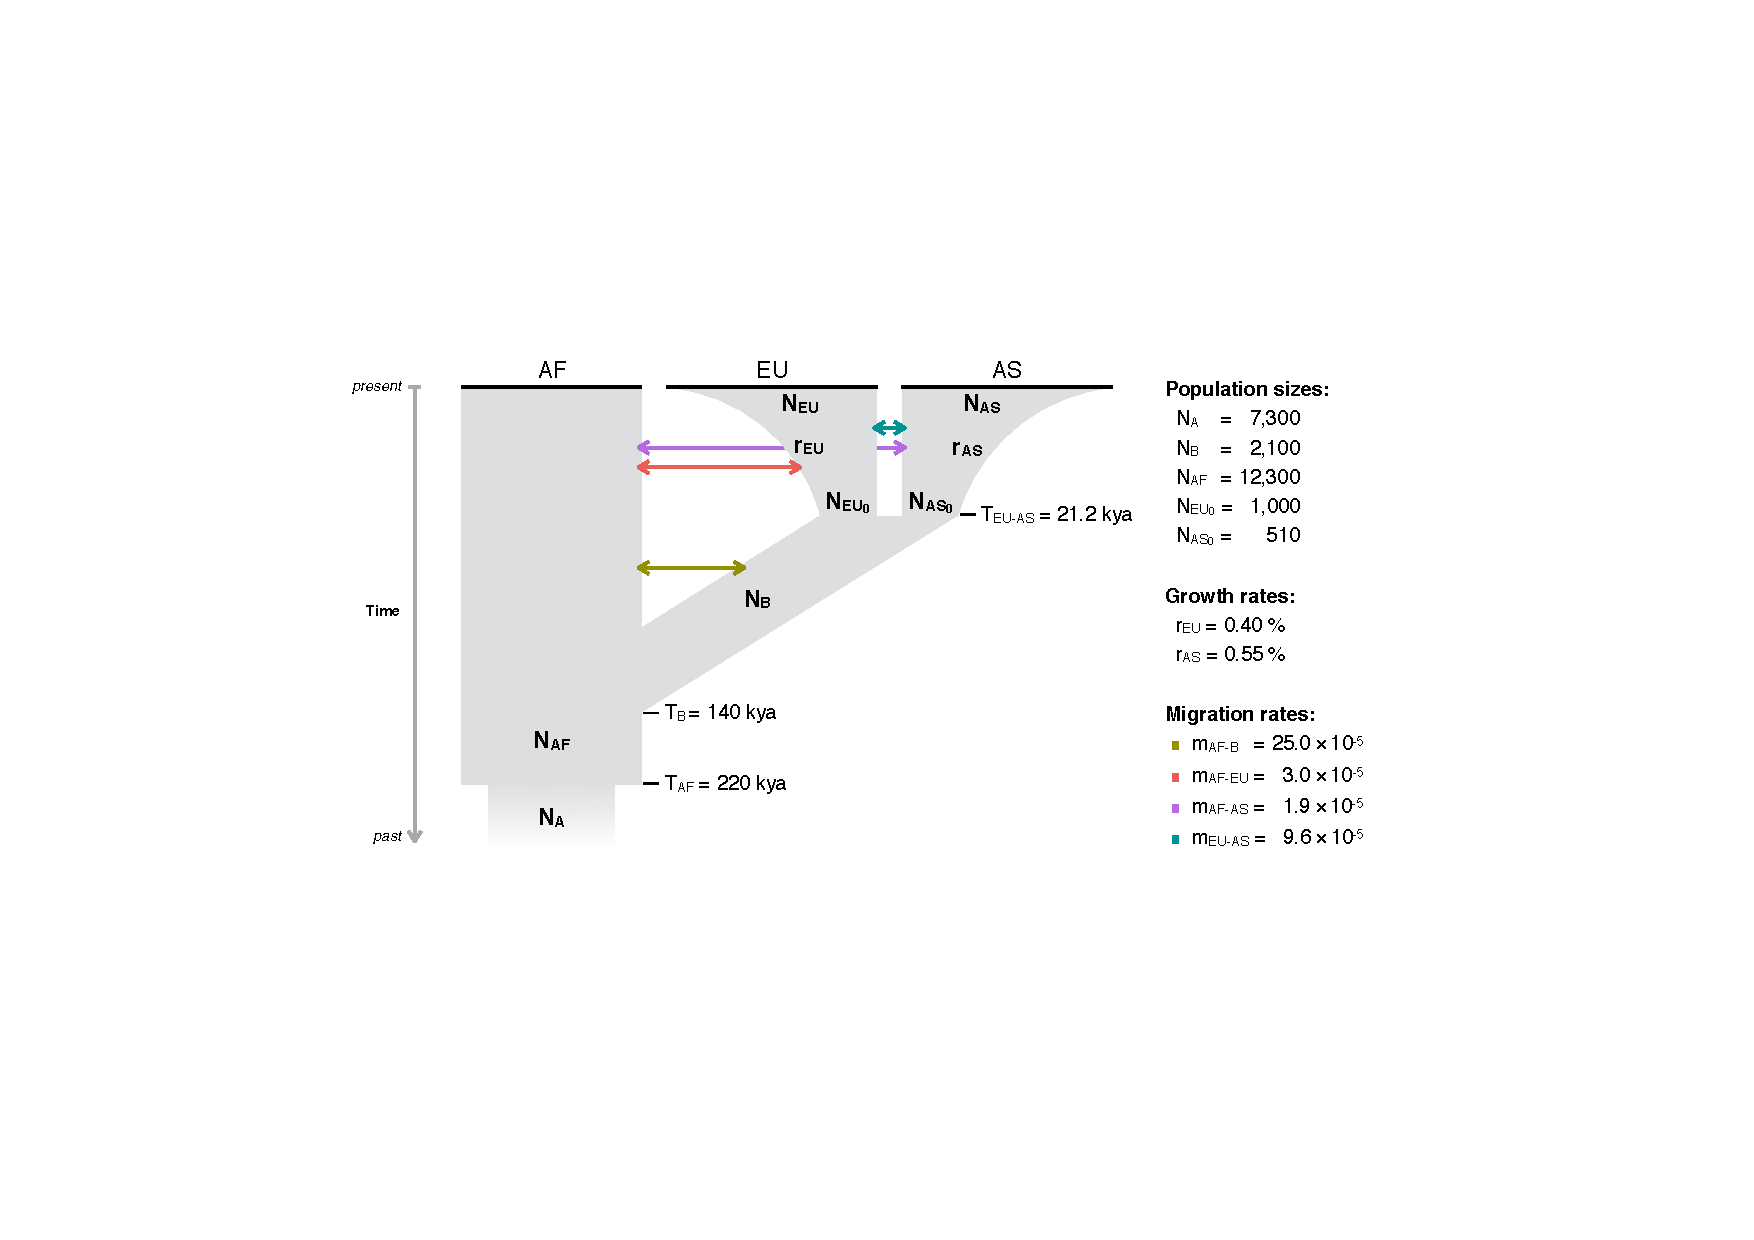
\includegraphics[width=0.95\textwidth]{./img/ch3/demo_model}
\Caption{Demographic model used in simulations}
{\N{3} populations were modelled, African (AF), European (EU), and Asian (AS), which derive from an ancestral population (A).
Both EU and AS experienced a bottleneck with subsequent exponential growth following the out-of-Africa expansion of a founder population (B) that split from the ancestral population.
Modified from \citet{Gutenkunst:2009gs}, Figure~2 (see \url{doi:10.1371/journal.pgen.1000695.g002}), with parameter values taken from Table~1 (see \url{doi:10.1371/journal.pgen.1000695.t001}).}
{fig:demo_model}
% \vspace{-5pt}
% \hrulefill%
\end{figure}
